\documentclass{tufte-handout}

% ams
\usepackage{amssymb,amsmath}

% utf8 encoding
\usepackage[utf8]{inputenc}

% graphix
\usepackage{graphicx}
\setkeys{Gin}{width=\linewidth,totalheight=\textheight,keepaspectratio}

% booktabs
\usepackage{booktabs}

% url
\usepackage{url}

% hyperref
\usepackage{hyperref}

% units.
\usepackage{units}

% pandoc syntax highlighting

% longtable

% multiplecol
\usepackage{multicol}

% lipsum
\usepackage{lipsum}

% title / author / date
\title{POLS 503: Omitted Variable Bias}
\author{Jeffrey Arnold}
\date{April 28, 2015}


\begin{document}

\maketitle



\section{Interpretations of
Regression}\label{interpretations-of-regression}

\begin{description}
\item[empirical]
descriptive association among variables.
\item[structural relation]
a causal relationship among variables
\end{description}

The issue of omitted variable bias only is meaningful when interpreting
the regression as a \emph{structural relationship}.

\section{Omitted Variable Bias}\label{omitted-variable-bias}

The regression \[
y = \beta_0 + \beta_1 X_1 + \beta_2 X_2
\]

Suppose that the correct specification is,\footnote{This could be
  derived for either the population or sample, although it is generally
  considered in the context of the latter.} \[
Y = \alpha + \beta_1 X_1 + \beta_2 X_2 + \epsilon
\] Now consider the regression in which the confounding covariate
\(X_2\) is ignored, \[
Y = \beta^*_0 + \beta^*_1 X_1 + \epsilon^*
\] What is the relationship between \(\beta_1\) and \(\beta^*_1\)? We
need the relationship between \(X_1\) and \(X_2\), \[
X_2 = \gamma_0 + \gamma_1 X_1 + \nu
\] Substituting the equation for \(X_2\) into the long equation, and
rearranging, yields \[
Y = (\beta_0 + \beta_2 \gamma_0) + (\beta_1 + \beta_2 \gamma_1) X_1 + (\epsilon_1 + \beta_2 \nu)
\] Thus, in the short equation \[
\beta^*_1 = \beta_1 + \beta_2 \gamma_1
\]

\begin{itemize}
\itemsep1pt\parskip0pt\parsep0pt
\item
  What is \(\gamma_1\) in terms of covariances and variances?
\item
  When \(\beta^*_1\) unbiased? (Two conditions)
\end{itemize}

Notes:

\begin{itemize}
\itemsep1pt\parskip0pt\parsep0pt
\item
  Means that if you claim no OVB, you are claiming you have the true
  model and vice versa.
\item
  Misspecification from the wrong functional form of \(X\)s or missing
  interactions is a form of OVB.
\item
  OVB is a deterministic relationship between coefficients and
  equations, it is not about sampling.
\item
  OVB little meaning outside of attempting to make causal claims about a
  \(\beta\).
\end{itemize}

\subsection{What to do about OVB}\label{what-to-do-about-ovb}

Control for more variables, e.g. ``kitchen sink''. Downside is loss of
efficiency (larger standard errors) in (1) degrees of freedom, and (2)
higher collinearity.

However, Clarke shows that adding variables does not \emph{necessarily}
decrease bias, and could increase it.

\newthought{The general advice} is to show robustness to specifications.

Compare the coefficient between a specification with no controls and
observed controls. The change in the coefficient due to observed
controls can be used to find plausible effects on the coefficient from
unobserved controls (omitted variables).

\subsection{When not to control for
variables}\label{when-not-to-control-for-variables}

\textbf{Do Not control for post-treatment variables}

Consider three variables \(X\), \(W\), and \(Y\). You are interested in
\(X \to Y\). \(W\) is

\begin{itemize}
\itemsep1pt\parskip0pt\parsep0pt
\item
  \emph{confounding} or \emph{lurking} if \(W \to X\) and \(W \to Y\)
\item
  \emph{indirect effect} if \(X \to W \to Y\)
\end{itemize}

Do not control for \emph{indirect effects}, these are part of the causal
effect.

In observational studies not always clear if a variable is
post-treatment or a control.

Example:

\begin{itemize}
\itemsep1pt\parskip0pt\parsep0pt
\item
  Effect of college on income. Do not control for occupation. Why?
\item
  Effect of post-college education on voting Democratic. Should we
  control for party ID? intention to vote 10 minutes before voting?
\end{itemize}

\begin{marginfigure}
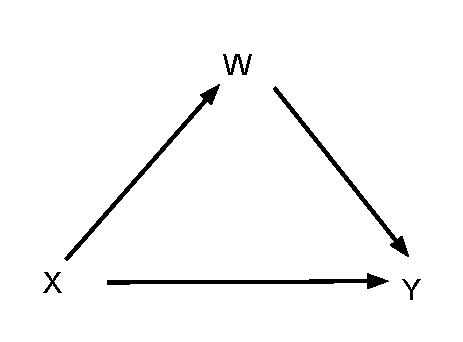
\includegraphics{images/Mediating_Variable_Diagram.pdf}
\caption{$W$ is an indirect effect of $X$ on $Y$}
\end{marginfigure}

\begin{marginfigure}
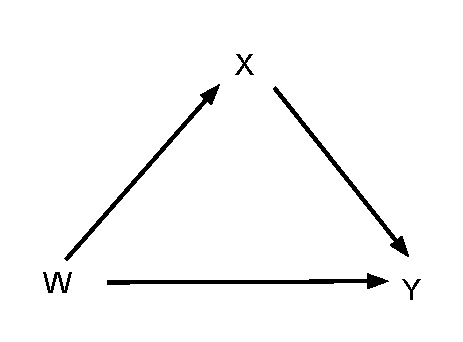
\includegraphics{images/Confounding_Variable_Diagram.pdf}
\caption{$W$ is a confounding variable of $X$ on $Y$}
\end{marginfigure}


\end{document}
